\documentclass[tikz]{standalone}

%outline around text
\usepackage[outline]{contour}
\contourlength{1.3pt}

%tikz
\usepackage{tikz}
\usetikzlibrary{knots, cd, calc}


\begin{document}
	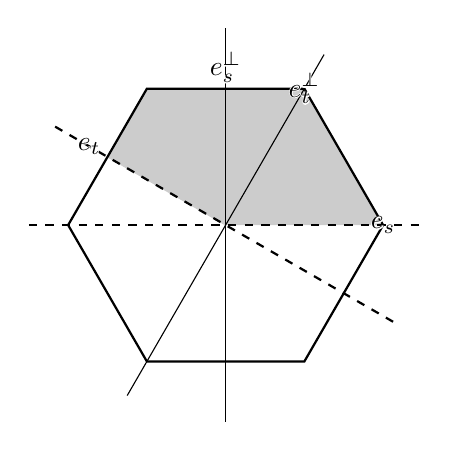
\begin{tikzpicture}[scale = 0.5]
		% hexagon
		\filldraw[color = black!20] 
			(4, 0) -- (60:4) 
				   -- (120:4) 
				   -- ($(120:4)!0.5!(180:4)$) 
				   -- (0, 0);
				   
		\draw[thick] 
			(4, 0) -- (60:4) 
				   -- (120:4) 
				   -- (180:4) 
				   -- (60:-4) 
				   -- (120:-4) 
				   -- (4, 0);
	
		\draw[thick, dashed] 
			(-5, 0) -- (5, 0);
			
		\draw[thick, dashed] 
			(150:5) -- (150:-5);
			
		\draw (0, -5) -- (0, 5);
		\draw (60:5) -- (60:-5);
	
		\node at (4, 0) {\contour{white}{$e_s$}};
		\node at (150:4) {\contour{white}{$e_t$}};
		\node at (60:4) {\contour{white}{$e_t^{\perp}$}};
		\node at (90:4) {\contour{white}{$e_s^\perp$}};
	\end{tikzpicture}
\end{document}